\chapter[Trabalhos Relacionados]{Trabalhos Relacionados}
\label{cap:trabalhosRelacionados}

Durante a pesquisa realizada para o desenvolvimento deste trabalho, foram encontrados alguns trabalhos que apresentam características semelhantes ao que foi proposto.
Neste capítulo, serão apresentados alguns desses trabalhos, para mostrar o que foi feito e como foi feito, além de mostrar as diferenças entre eles e o trabalho proposto.

O trabalho apresentado por \citeauthor{jogador_xadrez} (\citeyear{jogador_xadrez}) apresenta um sistema para jogar xadrez contra um computador utilizando um tabuleiro físico.
Neste trabalho, foi desenvolvido um tabuleiro modificado que utiliza motores de passo e um eletroímã para movimentar as peças, conforme apresentado na Figura \ref{fig:jogadorXadrez}.
Além disso, foi implementado um sistema de visão computacional para detectar qual peça foi movimentada pelo jogador.

\begin{figure}[H]
    \centering
    \caption{Jogador de Xadrez Robótico com Visão Computacional}
    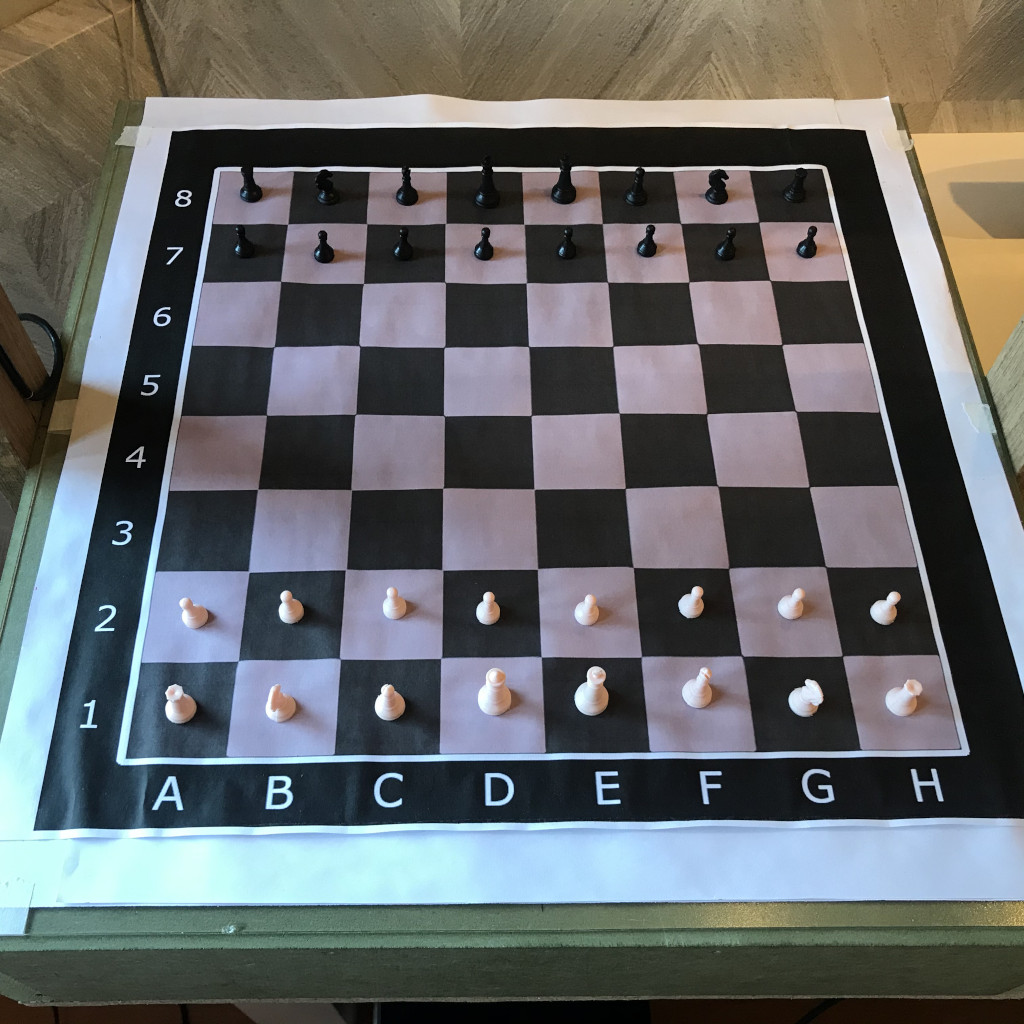
\includegraphics[keepaspectratio=true, width=0.6\textwidth]
    	{img/jogador-xadrez.jpg}
    \fonte{\citeauthor{jogador_xadrez} (\citeyear{jogador_xadrez})}
    \label{fig:jogadorXadrez}
\end{figure}

Em outra frente, o trabalho de \citeauthor{ferramenta_braco_robotico} (\citeyear{ferramenta_braco_robotico}) apresenta uma ferramenta para manipular um braço robótico utilizando um computador.
Essa ferramenta recebe os ângulos desejados de cada junta do braço e realiza o movimento, utilizando-se de cinemática direta, conforme apresentado na Figura \ref{fig:ferramentaComputacional}.
Lançando-se mão dessa ferramenta, é possível movimentar o braço robótico com base nos ângulos,
entretanto não é possível diretamente definir sua posição final.

\begin{figure}[H]
    \centering
    \caption{Uma Ferramenta Computacional para Manipulação de um Braço Robótico}
    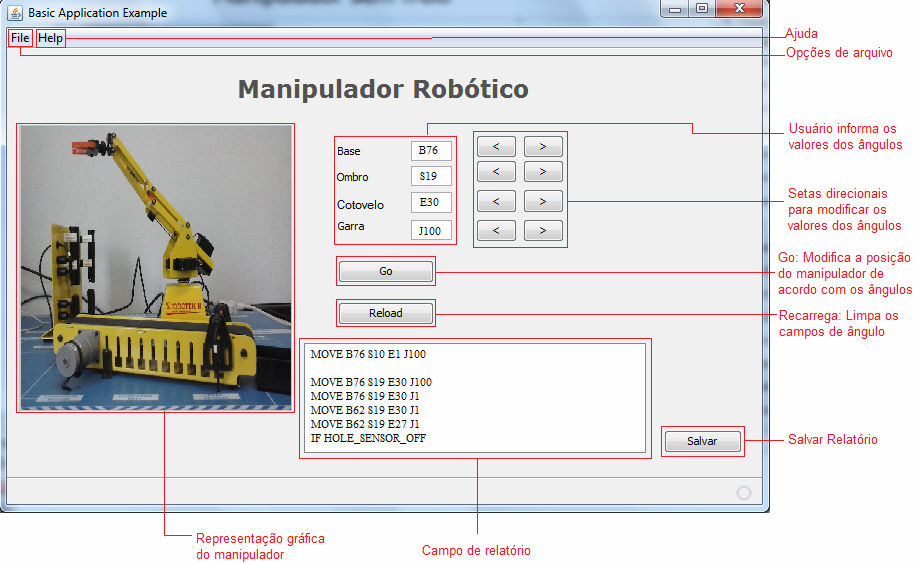
\includegraphics[keepaspectratio=true, width=0.95\textwidth]
    	{img/ferramenta-computacional.jpg}
    \fonte{\citeauthor{ferramenta_braco_robotico} (\citeyear{ferramenta_braco_robotico})}
    \label{fig:ferramentaComputacional}
\end{figure}

\citeauthor{inverse_kinematics_five_joint} (\citeyear{inverse_kinematics_five_joint}) apresenta um estudo sobre cinemática inversa de um braço robótico de cinco juntas.
Neste trabalho, é apresentado um método para calcular os ângulos de cada junta, com base na posição final desejada.
A partir desse método, é possível movimentar o braço robótico com mais facilidade, pois não é necessário calcular os ângulos manualmente.

A partir do estudo desses trabalhos, foi possível definir o escopo do trabalho proposto e observar as diferenças em relação aos trabalhos relacionados.
O trabalho proposto implementa o jogo de xadrez, assim como o trabalho de \citeauthor{jogador_xadrez} (\citeyear{jogador_xadrez}), porém utiliza um braço robótico para movimentar as peças.
Para isso, foi necessário desenvolver uma ferramenta que permite a comunicação entre um computador e o braço robótico, assim como o trabalho de \citeauthor{ferramenta_braco_robotico} (\citeyear{ferramenta_braco_robotico}). 
Por sua vez, o controle do braço é feito através de um sistema de cinemática inversa, assim como o trabalho de \citeauthor{inverse_kinematics_five_joint} (\citeyear{inverse_kinematics_five_joint}), porém com um menor número de juntas.